



\begin{frame}
		\frametitle{IC}
		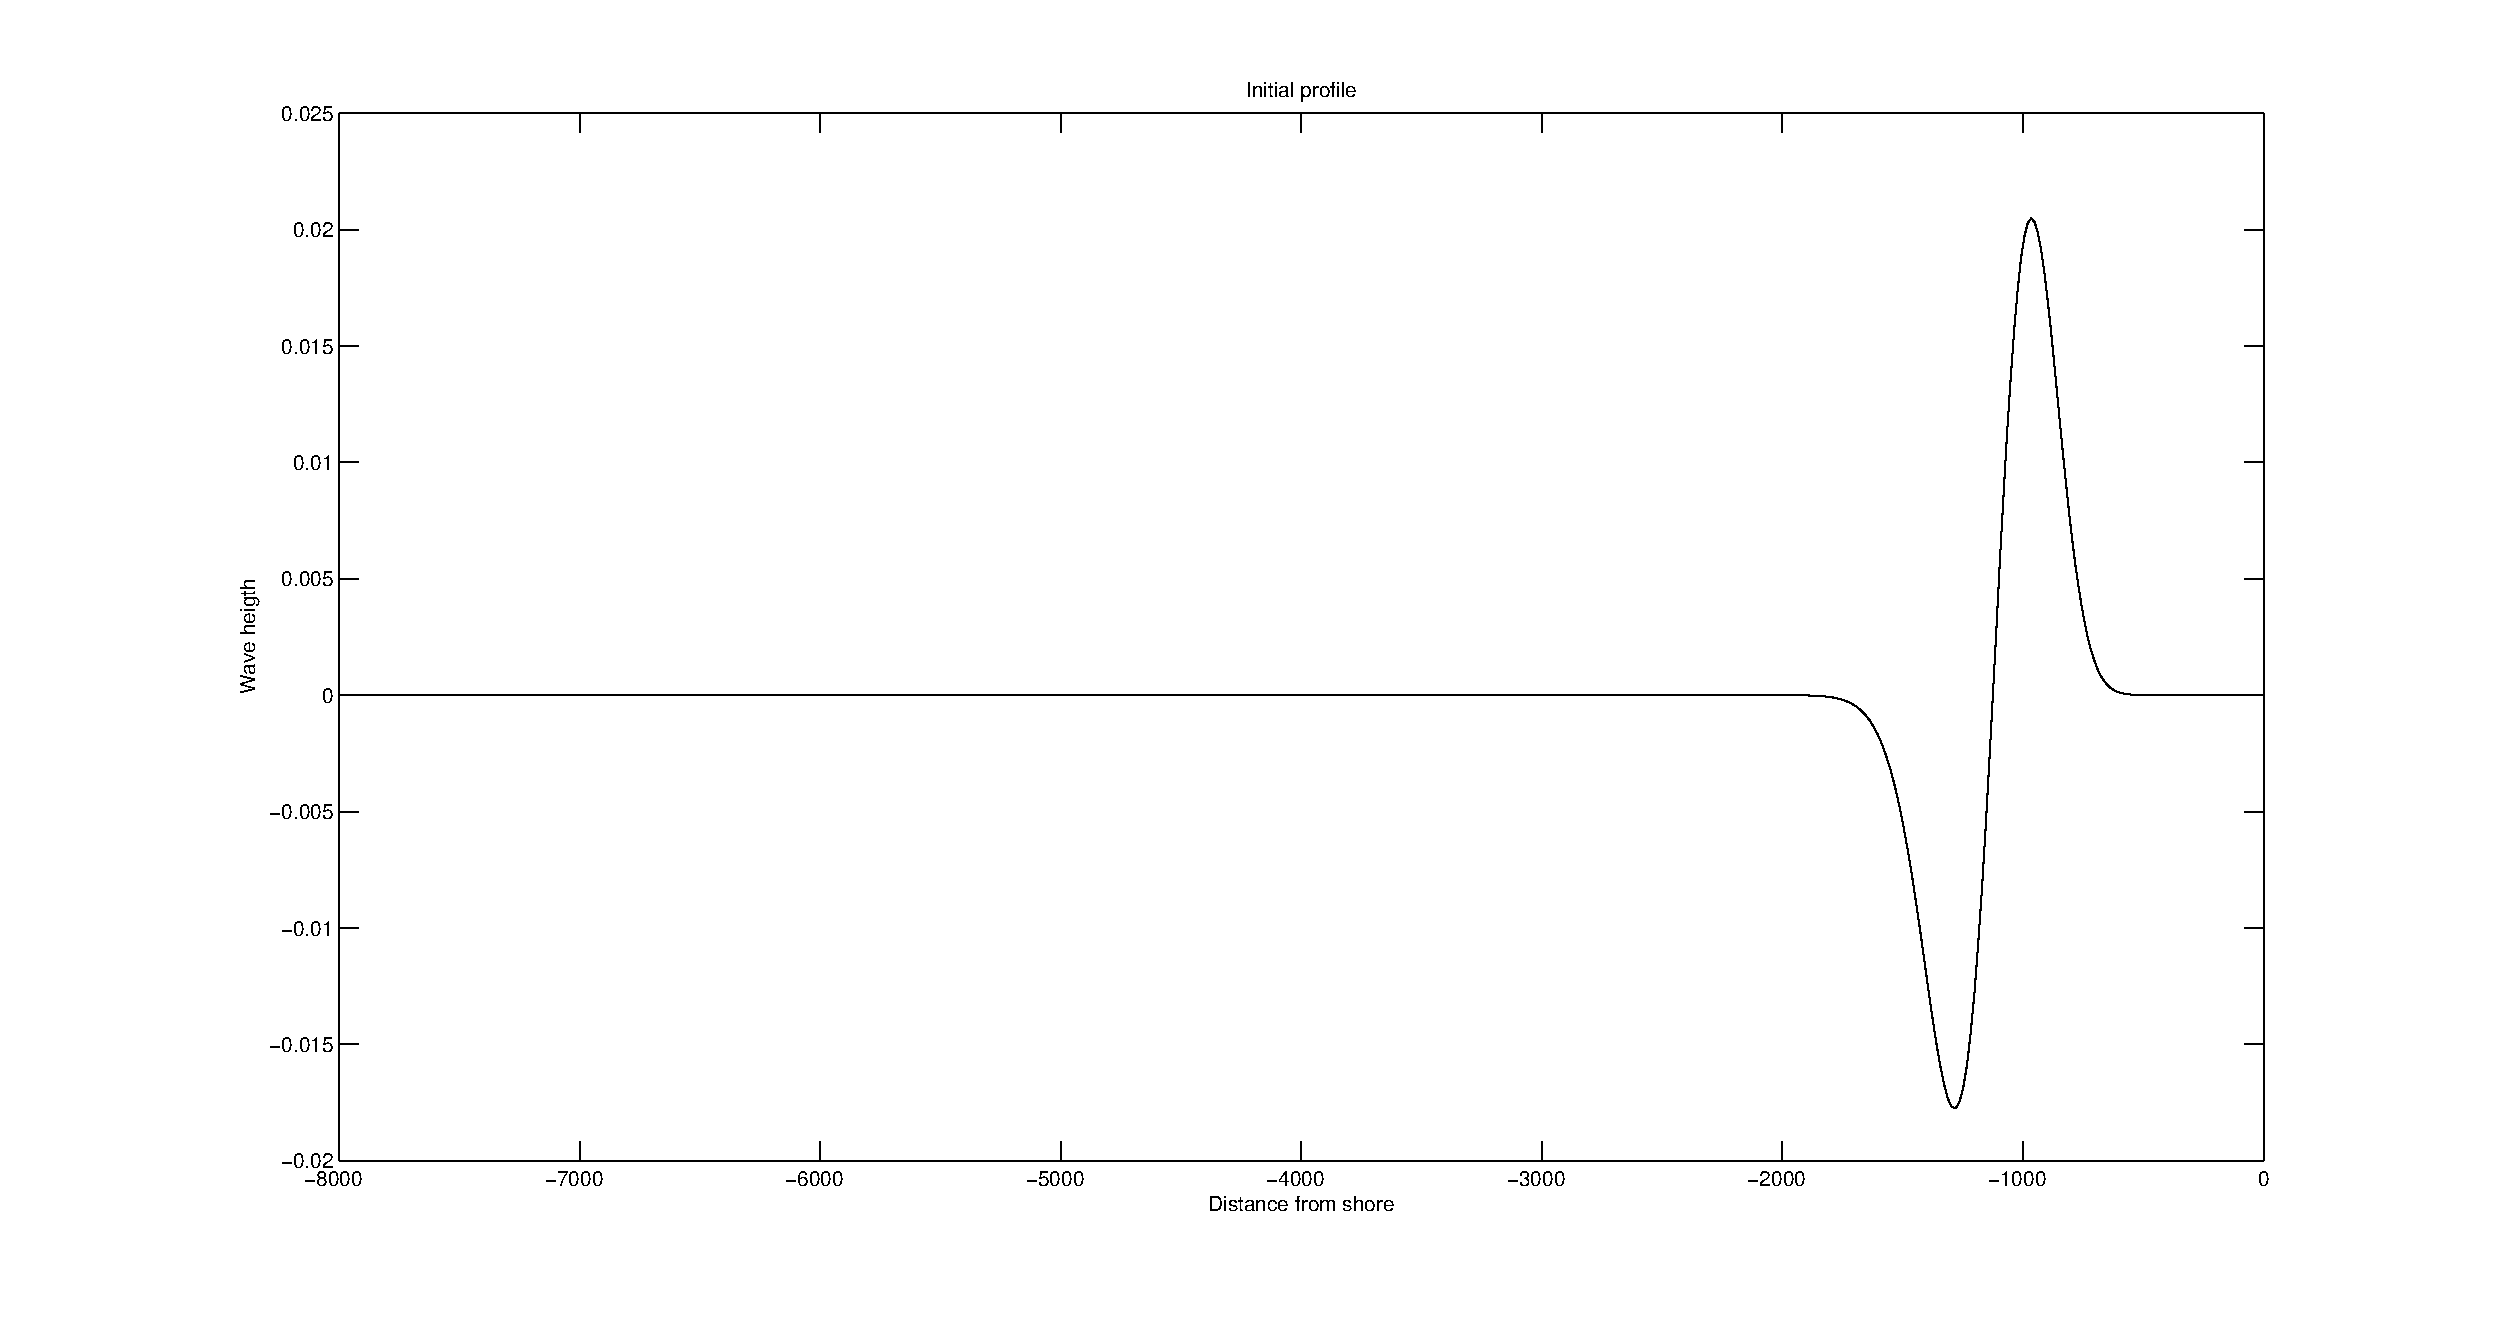
\includegraphics[width=\textwidth]{IC.eps}
		\end{frame}

\begin{frame}
		\frametitle{Eigen values}
		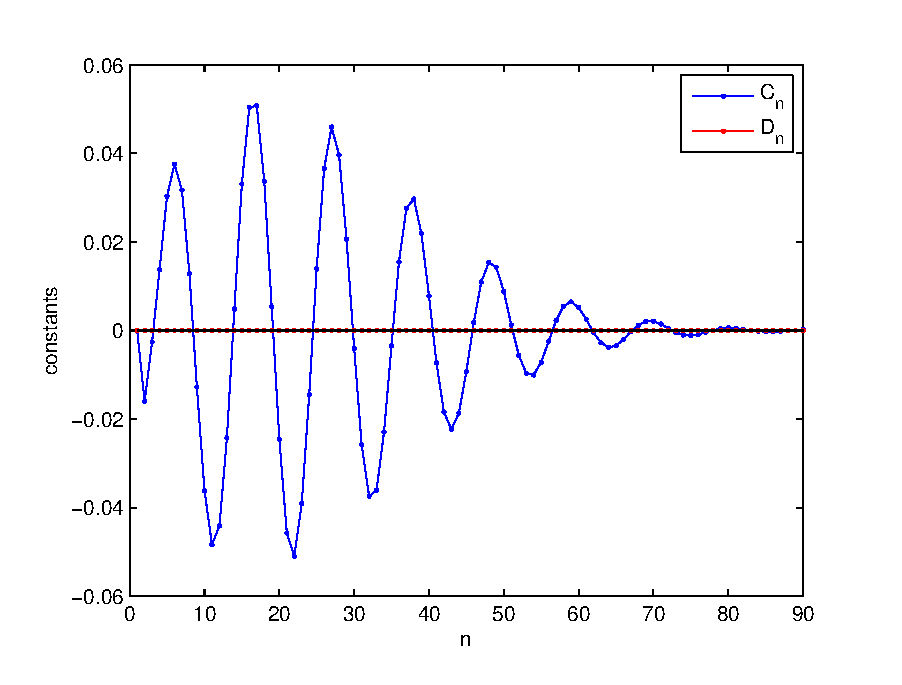
\includegraphics[width=\textwidth]{Const.eps}
		\end{frame}

	
	
				\begin{frame}
		\frametitle{Eigen Functions}
		\begin{tabular}{|c|c|}\hline
		\includegraphics[width=.45\textwidth]{Eigenfunctions1.png}&\includegraphics[width=.45\textwidth]{Eigenfunctionsx1.png}\\\hline
		\includegraphics[width=.45\textwidth]{Eigenfunctions2.png}&\includegraphics[width=.45\textwidth]{Eigenfunctionsx2.png}\\\hline
		\end{tabular}
		
	\end{frame}
	
	
	
	
		
	\begin{frame}
		\frametitle{Numerical error in max run-up}
		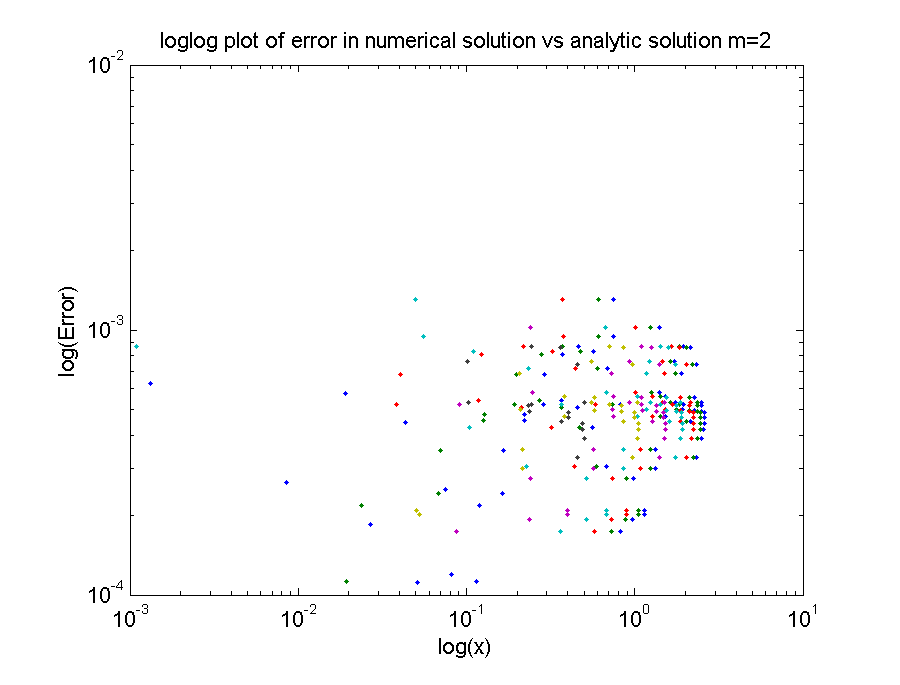
\includegraphics[width=\textwidth]{Error.eps}
		
	\end{frame}
	
	
	\begin{frame}
		\frametitle{Error in boundary assumption}
		\centering
		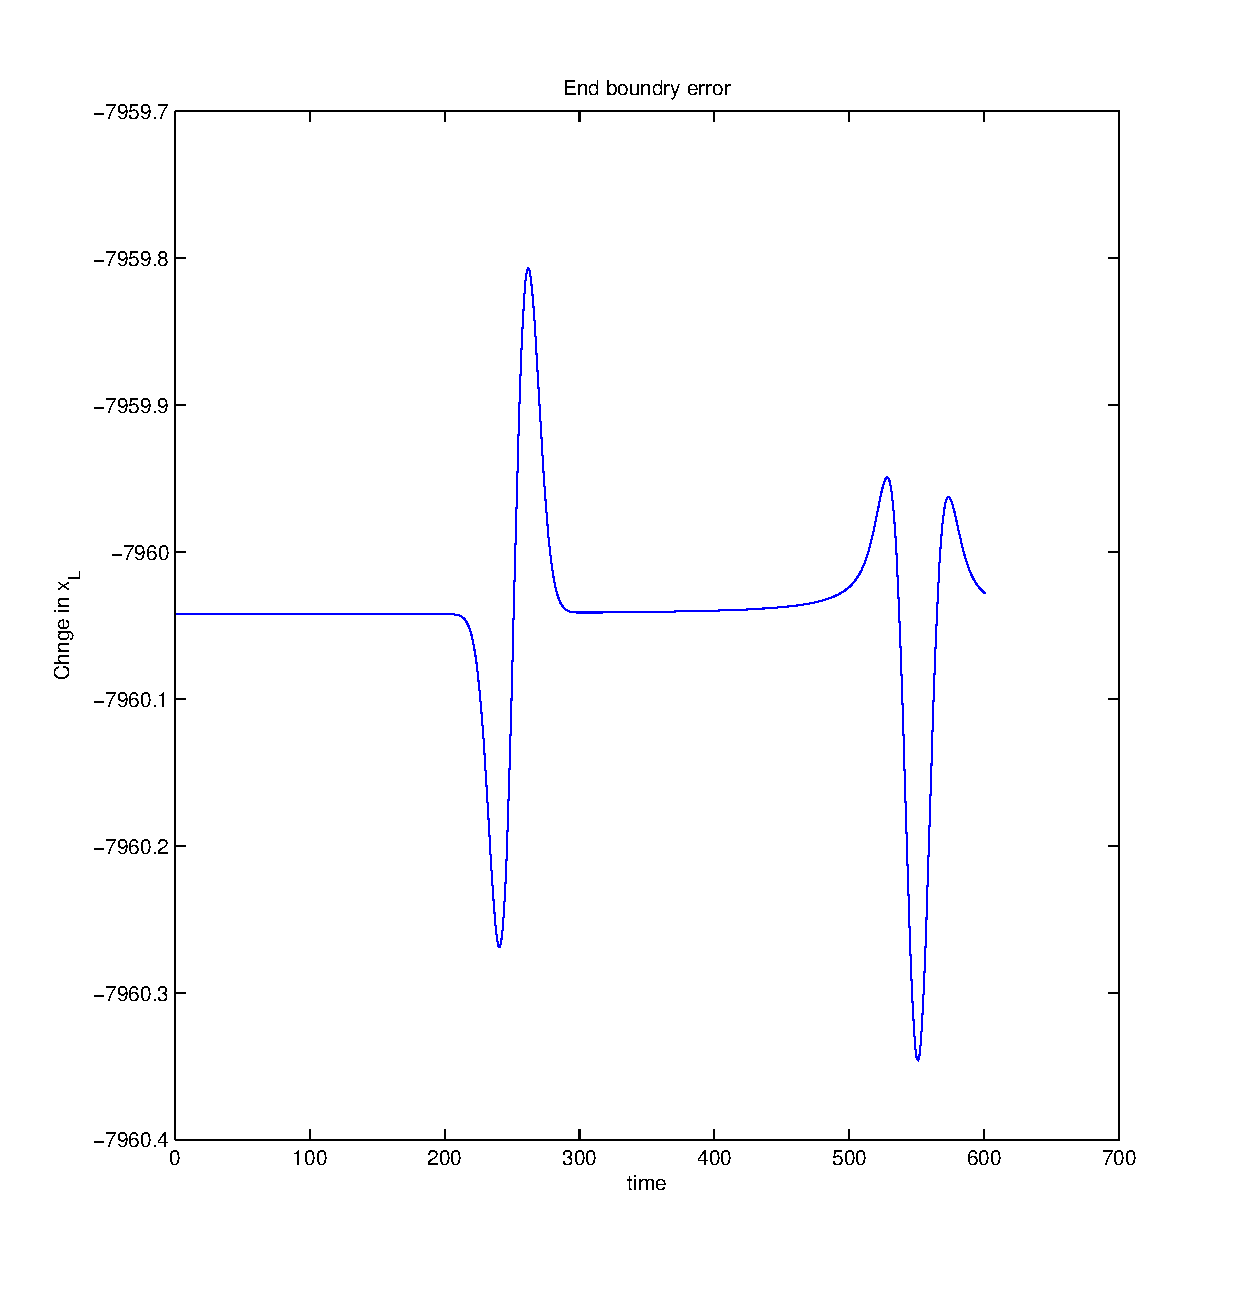
\includegraphics[width=.7\textwidth]{x_l.eps}
		
	\end{frame}
	
	
	
	
		\begin{frame}
		\frametitle{Effect of $m$ on run-up}
		\centering
		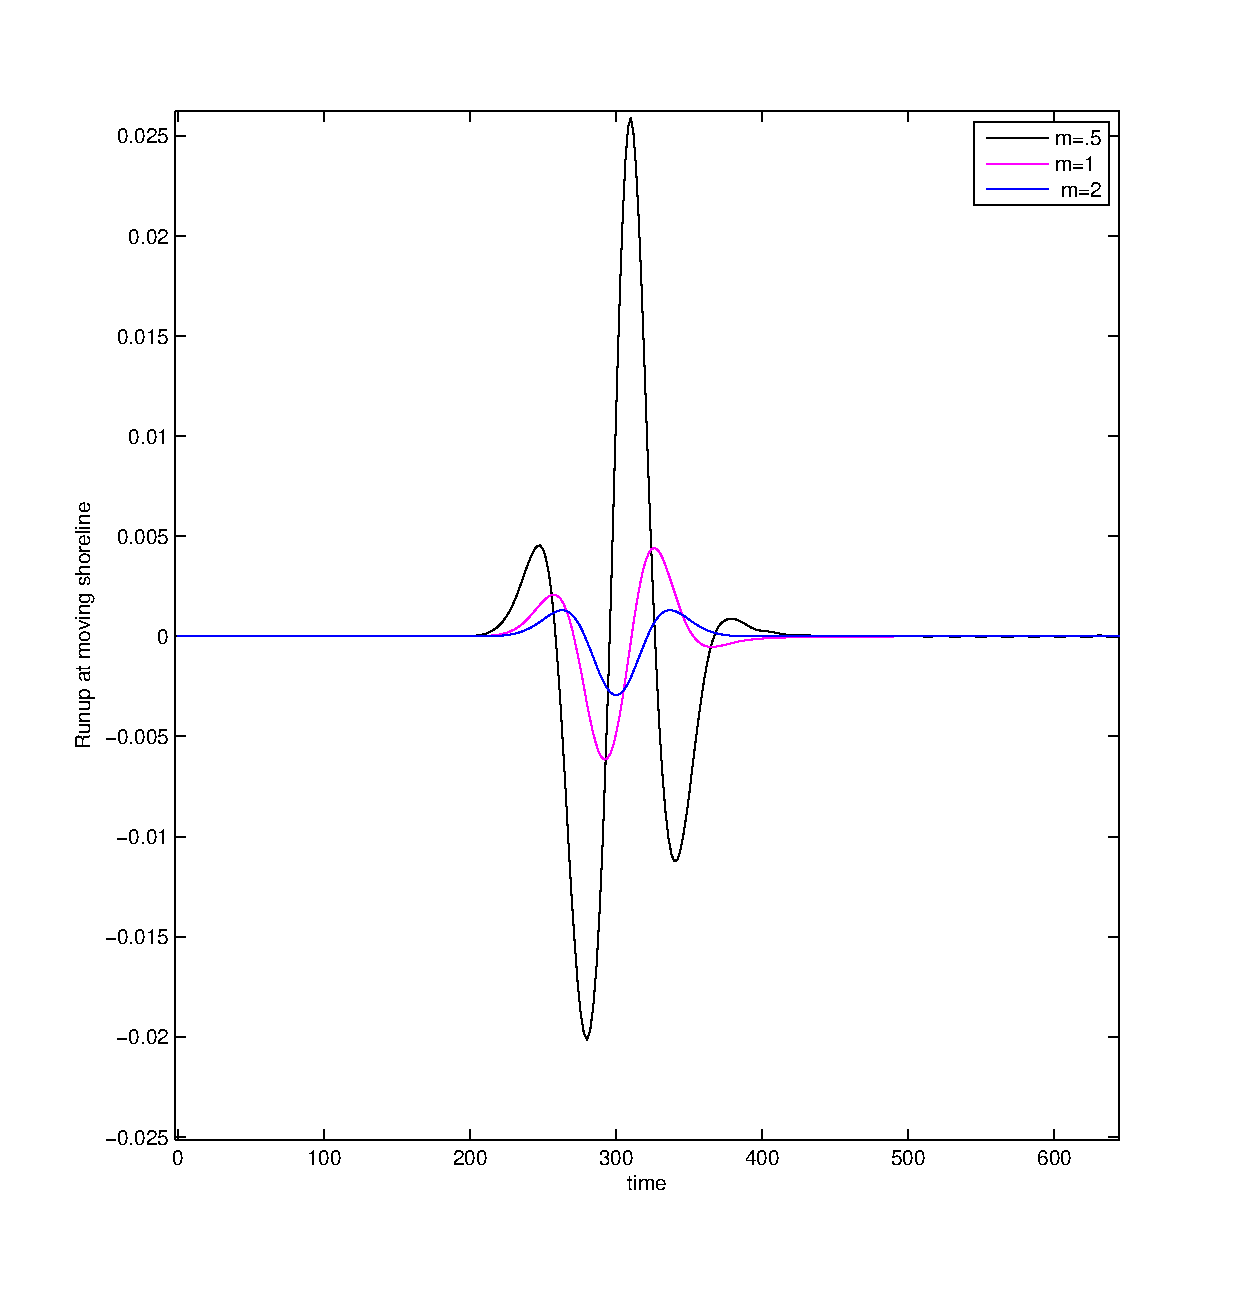
\includegraphics[width=.7\textwidth]{Runup.eps}
		
	\end{frame}
	
			\begin{frame}
		\frametitle{Effect of $m$ on run-up 2}
		\centering
		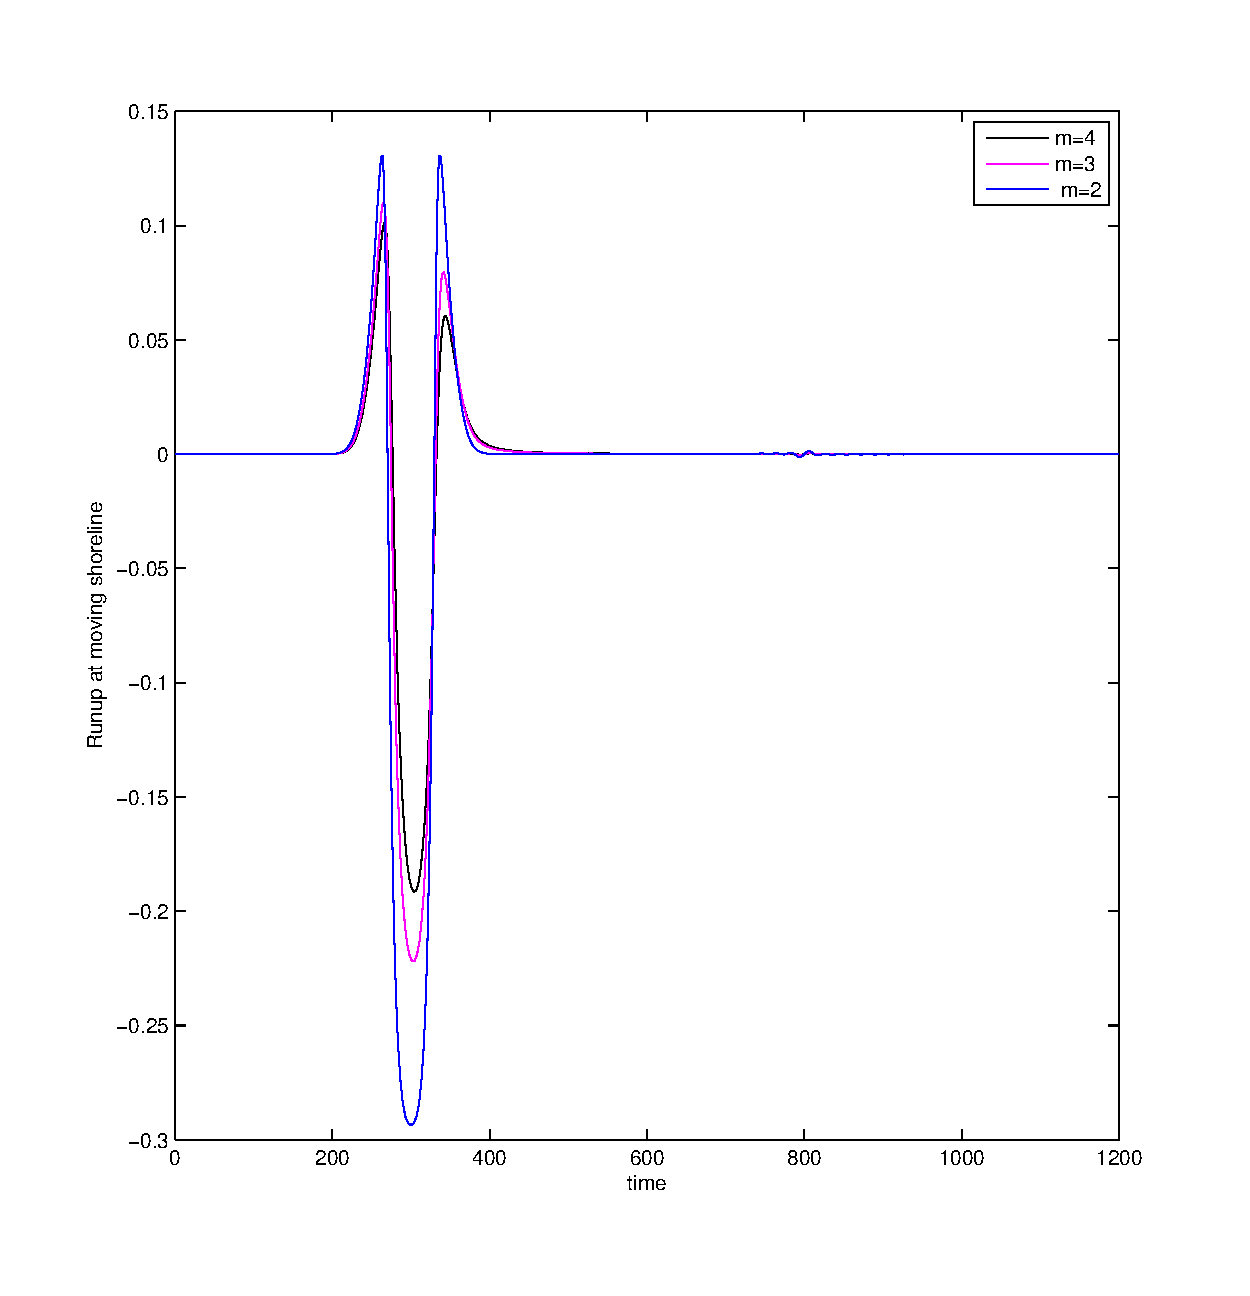
\includegraphics[width=.7\textwidth]{Runup2.eps}
		
	\end{frame}
	
